\documentclass[uplatex]{jsarticle} %titlepage
\usepackage[dvipdfmx]{graphicx}
\usepackage{float}

\title{聴覚による没入感}
\author{C0118005 A3 秋本 遥基}
\date{}

\begin{document}
\maketitle

\section{仮想現実感}

  両耳に届く音量差や時間差だけでは前後や上下を判別できない理由としては、耳に入ってくる音声のみを想定しており、本来耳周辺に伝わる音(音波)が想定されていないためである。以下の図\ref{fig}(引用:\cite{item})のように耳周辺の頭部にぶつかるであろう音波も考慮せねばならない。(参考:\cite{sour})

\begin{figure}[H]
  \centering
  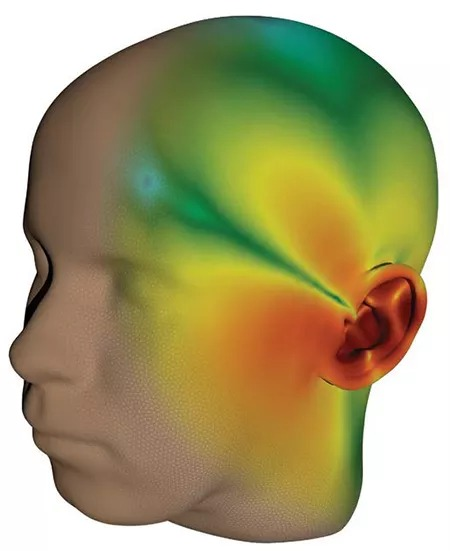
\includegraphics[scale= 0.3]{./mimi.jpg}
  \caption{頭部に当たる波の強さ}
  \label{fig}
\end{figure}

\begin{thebibliography}{99}
  \bibitem{sour} \verb+アクティブラーニングで学ぶ 情報リテラシー,コロナ社+
  \bibitem{item} \verb+https://www.tvtechnology.com/opinions/deriving-hrtfs-and-the-aes692015-file-format+
\end{thebibliography}

\end{document}
